\documentclass{article}
\usepackage{amsmath}
\usepackage{amssymb}
\usepackage{graphicx}
\usepackage{hyperref}
\usepackage{algorithm}
\usepackage{algpseudocode}
\usepackage{booktabs}
\usepackage{tikz}
\usepackage{color}

\title{Advanced Mathematical Concepts in Local Regression Methods}
\author{Michael Lee}
\date{\today}

\begin{document}

\maketitle

\section{Introduction}

This document provides detailed explanations of key mathematical concepts used in the PyDelt library's local regression methods. We focus on three fundamental concepts that are essential for understanding the implementation of derivative estimation techniques:

\begin{itemize}
    \item Polynomial basis functions
    \item Gram-Schmidt orthogonalization
    \item Weight matrix calculation
\end{itemize}

These concepts are particularly important for understanding the GOLD (Generalized Orthogonal Local Derivative) and GLLA (Generalized Local Linear Approximation) methods.

\section{Polynomial Basis Functions}

\subsection{Basic Concept}

Polynomial basis functions are a set of functions that can be linearly combined to represent polynomials of various degrees. The standard polynomial basis is:

\begin{equation}
\{1, x, x^2, x^3, \ldots, x^n\}
\end{equation}

Each function in this set is a monomial of a specific degree. Any polynomial of degree $n$ or less can be expressed as a linear combination of these basis functions:

\begin{equation}
p(x) = a_0 \cdot 1 + a_1 \cdot x + a_2 \cdot x^2 + \ldots + a_n \cdot x^n = \sum_{i=0}^{n} a_i x^i
\end{equation}

\subsection{Role in Local Regression}

In local regression methods, polynomial basis functions serve several important purposes:

\begin{enumerate}
    \item \textbf{Local Approximation}: They allow us to approximate the behavior of a function within a small window using a polynomial of specified degree.
    
    \item \textbf{Taylor Series Connection}: They relate directly to the terms in a Taylor series expansion, where each term corresponds to a derivative of a specific order:
    
    \begin{equation}
    f(x) \approx f(x_0) + f'(x_0)(x-x_0) + \frac{f''(x_0)}{2!}(x-x_0)^2 + \ldots + \frac{f^{(n)}(x_0)}{n!}(x-x_0)^n
    \end{equation}
    
    \item \textbf{Derivative Estimation}: By fitting a polynomial to data points in a window, we can estimate derivatives by extracting the coefficients and applying appropriate scaling.
\end{enumerate}

\subsection{Implementation in PyDelt}

In the PyDelt library, polynomial basis functions are used in both the GLLA and GOLD methods. For example, in the GOLD method, we create a basis of polynomial functions:

\begin{equation}
\phi_k(t) = t^k \quad \text{for } k = 0, 1, \ldots, n
\end{equation}

This is implemented in the code as:

\begin{verbatim}
# Create basis functions (powers of t)
Xi = np.vstack([t**q for q in range(n+1)])
\end{verbatim}

Where `t` is a vector of time points centered around the middle point of the window, and `n` is the maximum order of derivative to estimate.

\subsection{Visual Representation}

Figure 1 shows the first few polynomial basis functions over the interval $[-1, 1]$.

\begin{center}
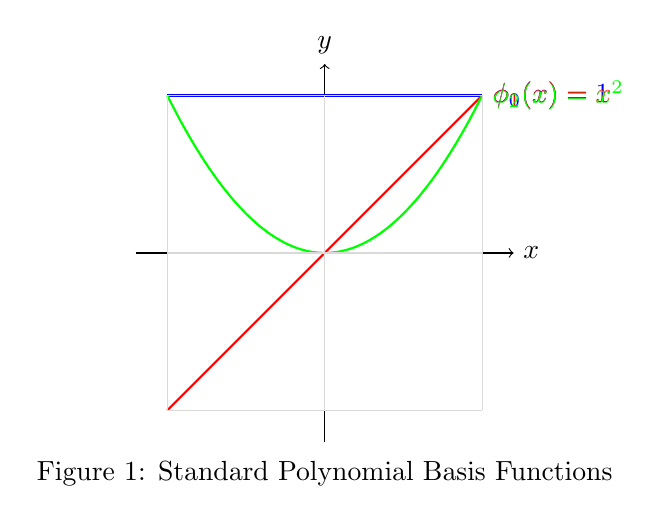
\begin{tikzpicture}[scale=2]
    \draw[->] (-1.2,0) -- (1.2,0) node[right] {$x$};
    \draw[->] (0,-1.2) -- (0,1.2) node[above] {$y$};
    
    % Plot the basis functions
    \draw[domain=-1:1, smooth, variable=\x, blue, thick] plot ({\x}, {1}) node[right] {$\phi_0(x) = 1$};
    \draw[domain=-1:1, smooth, variable=\x, red, thick] plot ({\x}, {\x}) node[right] {$\phi_1(x) = x$};
    \draw[domain=-1:1, smooth, variable=\x, green, thick] plot ({\x}, {\x*\x}) node[right] {$\phi_2(x) = x^2$};
    
    % Add grid
    \draw[gray!30] (-1,-1) grid (1,1);
    
    % Add labels
    \node at (0,-1.4) {Figure 1: Standard Polynomial Basis Functions};
\end{tikzpicture}
\end{center}

\section{Gram-Schmidt Orthogonalization}

\subsection{Basic Concept}

Gram-Schmidt orthogonalization is a procedure for converting a set of linearly independent vectors into a set of orthogonal vectors. Two vectors are orthogonal if their dot product is zero. An orthogonal basis has several desirable numerical properties, including improved stability in computational algorithms.

\subsection{The Process}

Given a set of linearly independent vectors $\{v_1, v_2, \ldots, v_n\}$, the Gram-Schmidt process produces an orthogonal set $\{u_1, u_2, \ldots, u_n\}$ as follows:

\begin{align}
u_1 &= v_1 \\
u_2 &= v_2 - \text{proj}_{u_1}(v_2) \\
u_3 &= v_3 - \text{proj}_{u_1}(v_3) - \text{proj}_{u_2}(v_3) \\
&\vdots \\
u_k &= v_k - \sum_{j=1}^{k-1} \text{proj}_{u_j}(v_k)
\end{align}

where $\text{proj}_u(v)$ is the projection of vector $v$ onto vector $u$, defined as:

\begin{equation}
\text{proj}_u(v) = \frac{\langle v, u \rangle}{\langle u, u \rangle} u
\end{equation}

and $\langle v, u \rangle$ is the inner product (dot product) of vectors $v$ and $u$.

\subsection{Simple Example}

Let's consider a simple example with two vectors in $\mathbb{R}^2$:
\begin{align}
v_1 &= (1, 0) \\
v_2 &= (1, 1)
\end{align}

Applying Gram-Schmidt:
\begin{align}
u_1 &= v_1 = (1, 0) \\
u_2 &= v_2 - \text{proj}_{u_1}(v_2) \\
&= (1, 1) - \frac{\langle (1, 1), (1, 0) \rangle}{\langle (1, 0), (1, 0) \rangle} (1, 0) \\
&= (1, 1) - \frac{1}{1} (1, 0) \\
&= (1, 1) - (1, 0) \\
&= (0, 1)
\end{align}

The result is an orthogonal basis $\{(1, 0), (0, 1)\}$, which in this case is the standard basis for $\mathbb{R}^2$.

\subsection{Application to Function Spaces}

The Gram-Schmidt process can be extended to function spaces, where the inner product is defined as:

\begin{equation}
\langle f, g \rangle = \int_a^b f(x)g(x) dx
\end{equation}

For discrete data points, this becomes:

\begin{equation}
\langle f, g \rangle = \sum_{i=1}^n f(x_i)g(x_i)
\end{equation}

\subsection{Implementation in PyDelt}

In the GOLD method, Gram-Schmidt orthogonalization is applied to the polynomial basis functions to create an orthogonal basis. This is implemented as:

\begin{verbatim}
# Gram-Schmidt orthogonalization of the basis functions
for q in range(1, n+1):
    for p in range(q):
        # Project higher order basis onto lower order and subtract
        Xi[q] -= np.dot(Xi[p], t**q) / np.dot(Xi[p], t**p) * Xi[p]
\end{verbatim}

This code orthogonalizes the polynomial basis functions $\{1, t, t^2, \ldots, t^n\}$ with respect to the discrete inner product defined by the points in the window.

\subsection{Benefits in Derivative Estimation}

Orthogonalization provides several benefits for derivative estimation:

\begin{itemize}
    \item \textbf{Numerical Stability}: Orthogonal bases lead to better-conditioned matrices, reducing numerical errors.
    
    \item \textbf{Independence of Estimates}: Each derivative order is estimated independently of the others, reducing error propagation.
    
    \item \textbf{Improved Accuracy}: Orthogonal polynomials often provide better approximations with fewer terms compared to standard polynomials.
\end{itemize}

\section{Weight Matrix Calculation}

\subsection{Basic Concept}

The weight matrix is a fundamental component in local regression methods that transforms data points in a window into derivative estimates. It encapsulates the mathematical relationship between the signal values and their derivatives based on the chosen basis functions.

\subsection{Mathematical Formulation}

In the context of derivative estimation, we want to find a matrix $W$ such that:

\begin{equation}
\hat{f}^{(k)}(x_0) = \sum_{i=1}^n W_{ki} f(x_i)
\end{equation}

where $\hat{f}^{(k)}(x_0)$ is the estimated $k$-th derivative at point $x_0$, and $f(x_i)$ are the function values at points $x_i$ in the window.

\subsection{Derivation}

The derivation of the weight matrix starts with the assumption that the function can be approximated by a linear combination of basis functions:

\begin{equation}
f(x) \approx \sum_{j=0}^n a_j \phi_j(x)
\end{equation}

where $\phi_j(x)$ are the basis functions (possibly orthogonalized) and $a_j$ are the coefficients to be determined.

Given a set of data points $(x_i, f(x_i))$ for $i = 1, 2, \ldots, m$, we can write this in matrix form:

\begin{equation}
\mathbf{f} = \Phi \mathbf{a}
\end{equation}

where $\mathbf{f} = [f(x_1), f(x_2), \ldots, f(x_m)]^T$, $\mathbf{a} = [a_0, a_1, \ldots, a_n]^T$, and $\Phi_{ij} = \phi_j(x_i)$.

The least squares solution for the coefficients is:

\begin{equation}
\mathbf{a} = (\Phi^T \Phi)^{-1} \Phi^T \mathbf{f}
\end{equation}

Now, the $k$-th derivative of the approximation at a point $x_0$ is:

\begin{equation}
f^{(k)}(x_0) \approx \sum_{j=k}^n a_j \frac{j!}{(j-k)!} \phi_{j-k}(x_0)
\end{equation}

In matrix form, this can be written as:

\begin{equation}
\mathbf{f}^{(k)}(x_0) = D_k \mathbf{a} = D_k (\Phi^T \Phi)^{-1} \Phi^T \mathbf{f}
\end{equation}

where $D_k$ is a matrix that transforms the coefficients into the $k$-th derivative.

The weight matrix is therefore:

\begin{equation}
W = D_k (\Phi^T \Phi)^{-1} \Phi^T
\end{equation}

\subsection{Implementation in PyDelt}

In the GOLD method, the weight matrix calculation is implemented as:

\begin{verbatim}
# Scale basis functions by factorial for derivative calculation
D = np.diag(1 / factorial(np.arange(n+1)))
# Apply scaling to orthogonalized basis
L = D @ Xi
# Calculate weights for derivative estimation
W = L.T @ np.linalg.inv(L @ L.T)
\end{verbatim}

Here:
\begin{itemize}
    \item `Xi` contains the orthogonalized basis functions evaluated at the points in the window
    \item `D` is a diagonal matrix with factorial scaling factors for each derivative order
    \item `L` is the scaled basis matrix
    \item `W` is the weight matrix that transforms signal values to derivative estimates
\end{itemize}

\subsection{Interpretation}

Each row of the weight matrix corresponds to a specific derivative order. When multiplied by the signal values in the window, it produces the estimate for that derivative order:

\begin{equation}
\hat{f}^{(k)}(x_0) = \sum_{i=1}^n W_{k+1,i} f(x_i)
\end{equation}

The weight matrix effectively acts as a finite difference scheme, but one that is optimally designed for the specific window and desired derivative orders.

\section{Practical Example: Estimating Derivatives}

Let's walk through a simple example to illustrate how these concepts work together to estimate derivatives.

\subsection{Setup}

Consider a function $f(x) = \sin(x)$ sampled at points $x = \{-0.2, -0.1, 0, 0.1, 0.2\}$, giving values $f = \{-0.199, -0.100, 0, 0.100, 0.199\}$ (approximately).

We want to estimate the first and second derivatives at $x = 0$ using a polynomial of degree 2.

\subsection{Step 1: Create the Basis Functions}

We use the polynomial basis $\{1, x, x^2\}$ evaluated at our sample points:

\begin{equation}
\Phi = \begin{bmatrix}
1 & -0.2 & 0.04 \\
1 & -0.1 & 0.01 \\
1 & 0 & 0 \\
1 & 0.1 & 0.01 \\
1 & 0.2 & 0.04
\end{bmatrix}
\end{equation}

\subsection{Step 2: Orthogonalize the Basis (Optional)}

For this simple example, we'll skip the orthogonalization step, but in practice, this would improve numerical stability.

\subsection{Step 3: Calculate the Weight Matrix}

The weight matrix is:

\begin{equation}
W = D (\Phi^T \Phi)^{-1} \Phi^T
\end{equation}

where $D$ is:

\begin{equation}
D = \begin{bmatrix}
1 & 0 & 0 \\
0 & 1 & 0 \\
0 & 0 & 2
\end{bmatrix}
\end{equation}

Computing this gives:

\begin{equation}
W \approx \begin{bmatrix}
0.2 & 0.2 & 0.2 & 0.2 & 0.2 \\
-0.5 & -0.25 & 0 & 0.25 & 0.5 \\
1 & -0.5 & -1 & -0.5 & 1
\end{bmatrix}
\end{equation}

\subsection{Step 4: Apply the Weight Matrix to the Function Values}

\begin{align}
\hat{f}(0) &= W_{1,:} \cdot f \approx 0.2 \cdot (-0.199) + 0.2 \cdot (-0.100) + 0.2 \cdot 0 + 0.2 \cdot 0.100 + 0.2 \cdot 0.199 \approx 0 \\
\hat{f}'(0) &= W_{2,:} \cdot f \approx -0.5 \cdot (-0.199) - 0.25 \cdot (-0.100) + 0 \cdot 0 + 0.25 \cdot 0.100 + 0.5 \cdot 0.199 \approx 1 \\
\hat{f}''(0) &= W_{3,:} \cdot f \approx 1 \cdot (-0.199) - 0.5 \cdot (-0.100) - 1 \cdot 0 - 0.5 \cdot 0.100 + 1 \cdot 0.199 \approx 0
\end{align}

These estimates match the true values of $\sin(0) = 0$, $\sin'(0) = \cos(0) = 1$, and $\sin''(0) = -\sin(0) = 0$.

\section{Conclusion}

Understanding polynomial basis functions, Gram-Schmidt orthogonalization, and weight matrix calculation is essential for grasping the mathematical foundations of the derivative estimation methods in PyDelt. These concepts work together to provide accurate and numerically stable estimates of derivatives from discrete data points.

The GOLD method, in particular, leverages these concepts to create an orthogonal basis that improves the accuracy and stability of derivative estimates. By applying the weight matrix derived from this basis to the signal values in a window, we can simultaneously estimate derivatives of multiple orders.

These techniques extend beyond derivative estimation and have applications in various fields, including signal processing, numerical analysis, and machine learning.

\end{document}
